\chapter{Conclusions}
Previous research and techniques relevant to the project were reviewed. In this part, some general animation techniques were briefly introduced. These include keyframe animation, procedural animation, kinematic animation and physical animation. The fundamentals of animation such as how to represent an object, animation control techniques and rendering were also included. Knowledge specifically for simulating an arthropod includes some biology knowledge, algorithms for simulating steps or paths and some possible implementations.
Analysis on possible solutions were given based on research of previous work. Project requirements, evaluation criteria were also set.  Planning including risk analysis and Gantt Chart was made after it.


The future work will mainly follow the Gantt Chart in the planning section. However, details may be changed due to risk of technical issues or time. The future work is generally described in figure \ref{fig:fw}. The work will be circulated until all the techniques were tested and embedded into the final system. The techniques testing mainly refers to implementation of a demo with a specific technique to be used in the project. The techniques testing is required because the techniques may be very hard to implement or cannot produce expected results. The merge phase mainly refer to integrate new module to the project. The documentation will be written after the whole project. 
\begin{figure}[ht!]
\centering
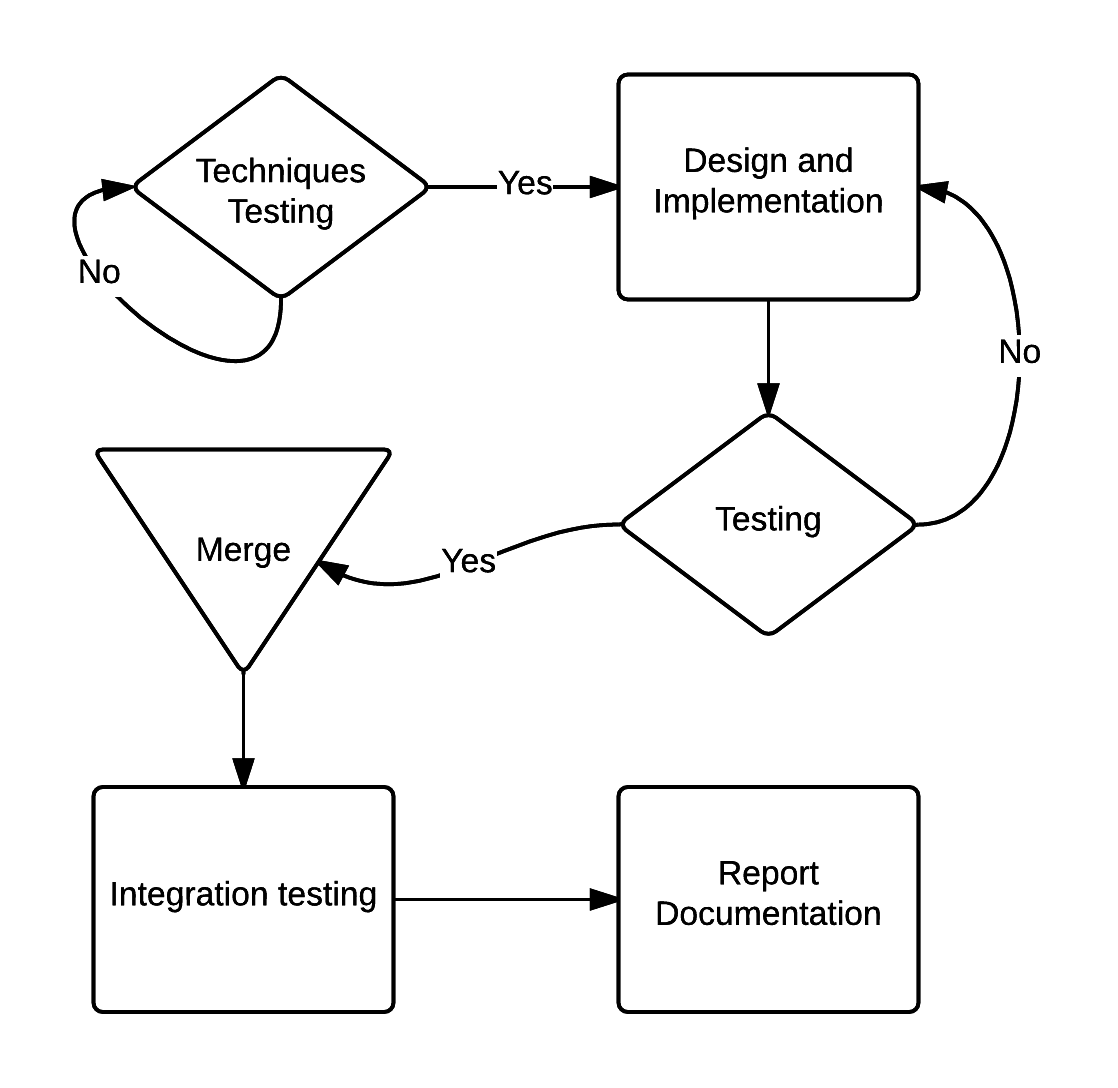
\includegraphics[width=10cm]{figures/fw.png}
\caption{Future work}
\label{fig:fw}
\end{figure}
